% ==== Gráfico de tiempos promedio (FM) ====
\begin{figure}[h!]
\centering
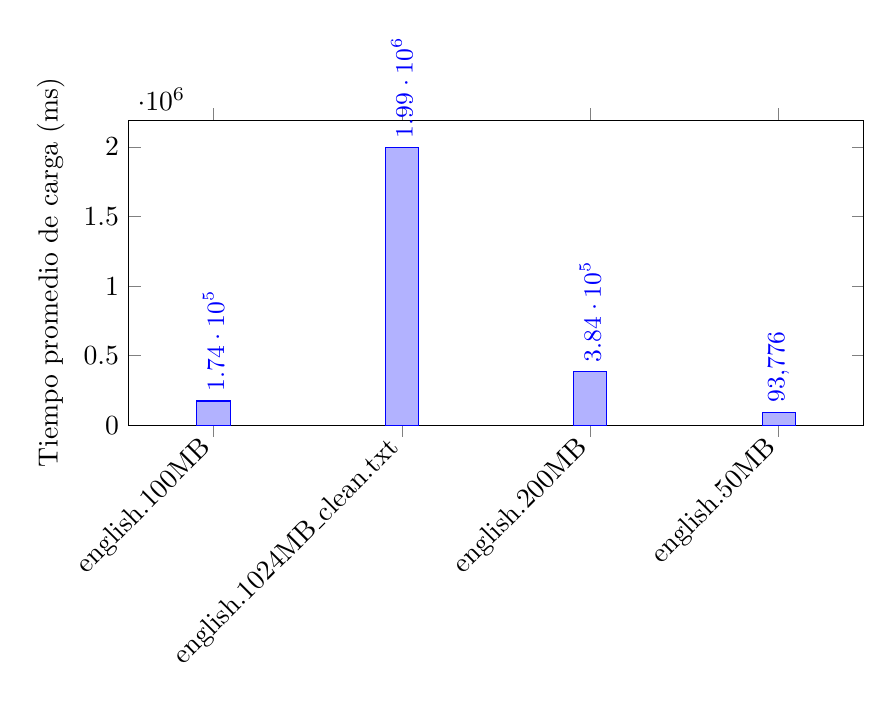
\begin{tikzpicture}
\begin{axis}[
    ybar,
    bar width=12pt,
    ylabel={Tiempo promedio de carga (ms)},
    symbolic x coords={english.100MB,english.1024MB\_clean.txt,english.200MB,english.50MB},
    xtick=data,
    x tick label style={rotate=45, anchor=east},
    ymin=0,
    width=0.9\textwidth,
    height=0.45\textwidth,
    nodes near coords,
    every node near coord/.append style={font=\small, rotate=90, anchor=west},
    enlarge x limits=0.15,
]
\addplot coordinates {
(english.100MB, 173567.40)
(english.1024MB\_clean.txt, 1994350.40)
(english.200MB, 383622.20)
(english.50MB, 93776.00)
};
\end{axis}
\end{tikzpicture}
\caption{Tiempo promedio de carga/creación para FM.}
\end{figure}
